\documentclass{article}
\usepackage[table,xcdraw]{xcolor} % Dla tabel
\usepackage{siunitx} % Provides the \SI{}{} and \si{} command for typesetting SI units
\usepackage{graphicx} % Required for the inclusion of images
\usepackage{natbib} % Required to change bibliography style to APA
\usepackage{amsmath} % Required for some math elements 
\setlength\parindent{12pt} % Removes all indentation from paragraphs
%\usepackage{times} % Uncomment to use the Times New Roman font
\usepackage{amsmath}
\usepackage[export]{adjustbox}
\usepackage{tikz}

\usepackage{pgfplots}
\usepackage[utf8]{inputenc} % Język polski
\usepackage{polski}
\usepackage[polish]{babel}

\usepackage[top=1in, bottom=1.25in, left=1.25in, right=1.25in]{geometry} % Marginesy
\usepackage{listings} % Kod programu
\usepackage{indentfirst} % Wcięcie przy pomocy \par
\usepackage{multicol} % Kilka kolumn dla itemize
\usepackage{color} % Kolorowanie tekstu
\usepackage{float}

%Projektowanie Efektywnych Algorytmów \\ {\normalsize Implementacja i analiza efektywności metody podziału i ograniczeń dla problemu komiwojażera}


%\renewcommand{\labelenumi}{\alph{enumi}.} % Zamienia litery w enumerate na a, b, c, ...
%----------------------------------------------------------------------------------------
%	DOCUMENT INFORMATION
%----------------------------------------------------------------------------------------
\title{Projektowanie Efektywnych Algorytmów \\ {\normalsize Implementacja i analiza efektywności Algorytmu Genetycznego dla problemu komiwojażera}}
\author{Sebastian Łągiewski 226173\\Łukasz Zatorski 226172 }

% Title page layout (fold)
\makeatletter
\renewcommand{\maketitle}{
	\begin{titlepage}
		\begin{center}
			\vspace*{3cm}
			\LARGE \@title \par
			\vspace{2cm}
			\textit{\small Autorzy:}\par
			\normalsize \@author\par \normalsize
			\vspace{3cm}
			Prowadzący : mgr inż. Radosław Idzikowski\\
			\vspace{3cm}
			Wydział Elektroniki\\ III rok \par
			\vspace{3cm}
			\small \@date
		\end{center}
	\end{titlepage}
}
\makeatother
\begin{document}
	\maketitle % Insert the title, author and date

%\begin{center}
%\begin{tabular}{l r}
%Data: & Semestr letni, 2017 \\ % Date the experiment was performed

%Prowadzący:  mgr inż. Radosław Idzikowski% Instructor/supervisor
%\end{tabular}
%\end{center}
\tableofcontents


% If you wish to include an abstract, uncomment the lines below
% \begin{abstract}
% Abstract text
% \end{abstract}

%----------------------------------------------------------------------------------------
%	SECTION 0
%----------------------------------------------------------------------------------------

%\newpage
%\section{Tytuł}} 
%\subsection{Tytuł}
%\par Tekst

%\begin{itemize}
%	\item\textit{Tekst} - Opis
%\end{itemize}

%\begin{enumerate}
%	\item Opis
%\end{enumerate}

%\begin{center}
%	\includegraphics[scale=0.6, center]{Screenshot_1.png}
%\end{center}

%\begin{lstlisting}[basicstyle=\small]
%	kod programu;
%\end{lstlisting}

%----------------------------------------------------------------------------------------
%	SECTION 1
%----------------------------------------------------------------------------------------
\newpage
\section{Opis algorytmu}
\par Algorytm genetyczny to rodzaj heurystyki przeszukującej przestrzeń  rozwiązań problemu w celu wyszukania rozwiązania optymalnego. Problem definiuje środowisko, w którym istnieje pewna populacja osobników. Każdy z osobników ma przypisany pewien zbiór informacji stanowiących jego genotyp, czyli konkretne rozwiązanie.
\newline
\newline
Pierwszym wymaganiem algorytmu genetycznego jest utworzenie populacji początkowej (losowego zbioru rozwiązań). Następnie N razy odbywa się selekcja, gdzie N oznacza rozmiar populacji rodzicielskiej - zaimplementowano wersję turniejową. W każdym turnieju bierze udział Q osobników, gdzie Q - rozmiar turnieju. W wyniku takiej selekcji otrzymujemy populację rodzicielską - grupę osobników, które będą poddawane krzyżowaniu - w zaimplementowanym algorytmi użyto operatora OX. Po skrzyżowaniu, każdy osobnik z określonym prawdopodobieństwem Pm może podlegać mutacji, czyli losowemu zdeformowaniu rozwiązania. W opisywanym algorytmie zaimplementowano dwie metody krzyżowania - swap oraz invert.
Warunkiem zakończenia algorytmu jest upływ określonego czasu.

\newpage
\section{Plan eksperymentu}
\subsection{Główne założenia}
\begin{itemize}
	\item Pomiar czasu został wykonany za pomocą klasy StopWatch(QueryPerformanceCounter).
	\item Do reprezentacji odległości między miastami użyto macierzy sąsiedztwa.
	\item Dla każdego z typów pomiaru algorytm wykonywany był 30 razy, wyniki uśredniono.
	\item Do przechowywania obecnej populacji użyto \textit{List} o zadeklarowanej stałej wielkości.
\end{itemize}

\subsection{Dobór parametrów}
\begin{itemize}
	\item Dla badań w zależności od rozmiaru populacji wybrano wartości: $<$ 50, 100, 500, 750, 1000, 1500, 2000 $>$, dla rozmiaru populacji macierzystej rozmPopulacji/2, rozmiaru turnieju = 20, oraz prawdopodobieństwu mutacji = 1\%, przy ilości miast = 226.
	\item Dla badań w zależności od rozmiaru populacji macierzystej wybrano wartości: $<$ 100, 250, 500, 750 $>$, dla rozmiaru populacji = 1000, rozmiaru turnieju = 20, oraz prawdopodobieństwu mutacji = 1\%, przy ilości miast = 403.
	\item Dla badań w zależności od rozmiaru turnieju wybrano wartości: $<$ 2, 5, 10, 20, 50, 100, 500 $>$, dla rozmiaru populacji = 1000, dla rozmiaru populacji macierzystej = 500, oraz prawdopodobieństwu mutacji = 1\%, przy ilości miast = 403.
	
\end{itemize}

\newpage
\section{Wyniki}
\subsection{Wpływ rozmiaru populacji na działanie algorytmu}
\begin{figure}[H]
	\begin{adjustbox}{addcode={\begin{minipage}{\width}}{\caption{%
						Wpływ rozmiaru populacji na jakość rozwiązania z biegiem czasu. Badania przeprowadzono dla instancji pr226.
			}\end{minipage}},rotate=90,center}
		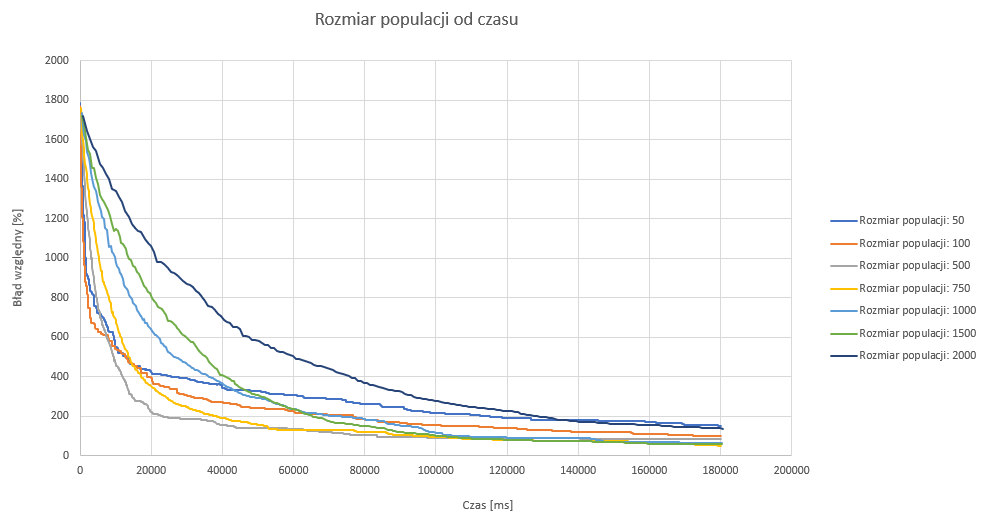
\includegraphics[scale=.55]{population.png}%
	\end{adjustbox}

	\begin{adjustbox}{angle=90, center}
		
		\begin{tabular}{|c|c|}
			\hline
			\multicolumn{1}{|c|}{\textbf{Roz. pop.}} & \textbf{Błąd wzgl. [\%]}  \\ \hline
			{50}                                	& 148,1              \\ \hline
			{100}                                & 100,16              \\ \hline
			{500}                                & 82,43                \\ \hline
			{750}                                & 47,72                \\ \hline
			{1000}                                & 62,28                \\ \hline
			{1500}                                & 58,25                 \\ \hline
			{2000}                                & 136,68                 \\ \hline
			
		\end{tabular}
		
	\end{adjustbox}
\end{figure}



\subsection{Wpływ rozmiaru populacji macierzystej na działanie algorytmu}
\begin{figure}[H]
	\begin{adjustbox}{addcode={\begin{minipage}{\width}}{\caption{%
						Wpływ rozmiaru populacji macierzystej na jakość rozwiązania z biegiem czasu. Badania przeprowadzono dla instancji rbg403.
			}\end{minipage}},rotate=90,center}
		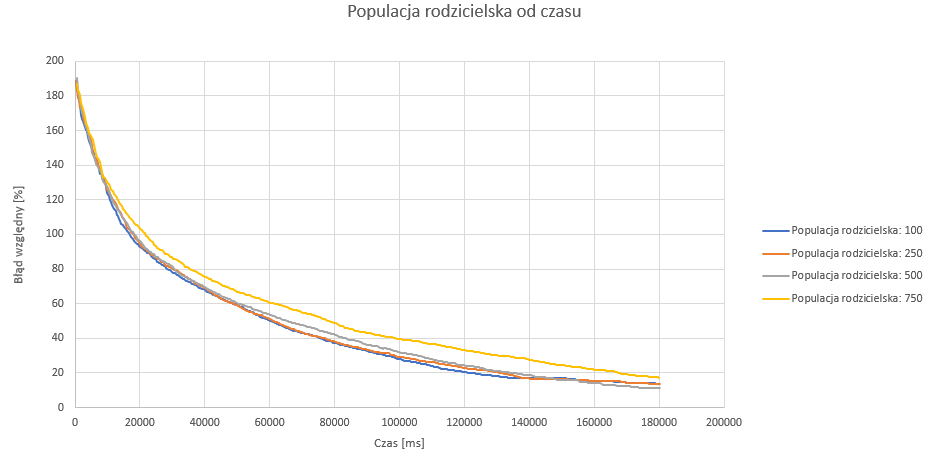
\includegraphics[scale=.59]{matingPool.png}%
	\end{adjustbox}
	\begin{adjustbox}{angle=90, center}
	
	\begin{tabular}{|c|c|}
		\hline
		\multicolumn{1}{|c|}{\textbf{Rozm. pop. rodz.}} & \textbf{Błąd wzgl. [\%]}  \\ \hline
		{100}                                	& 13,83              \\ \hline
		{250}                                & 13,75              \\ \hline
		{500}                                & 10,99               \\ \hline
		{750}                                & 17,07                \\ \hline		
	\end{tabular}
	
	\end{adjustbox}
\end{figure}

\subsection{Wpływ rozmiaru turnieju na działanie algorytmu}
\begin{figure}[H]
	\begin{adjustbox}{addcode={\begin{minipage}{\width}}{\caption{%
						Wpływ rozmiaru turnieju na jakość rozwiązania z biegiem czasu. Badania przeprowadzono dla instancji rbg403.
			}\end{minipage}},rotate=90,center}
		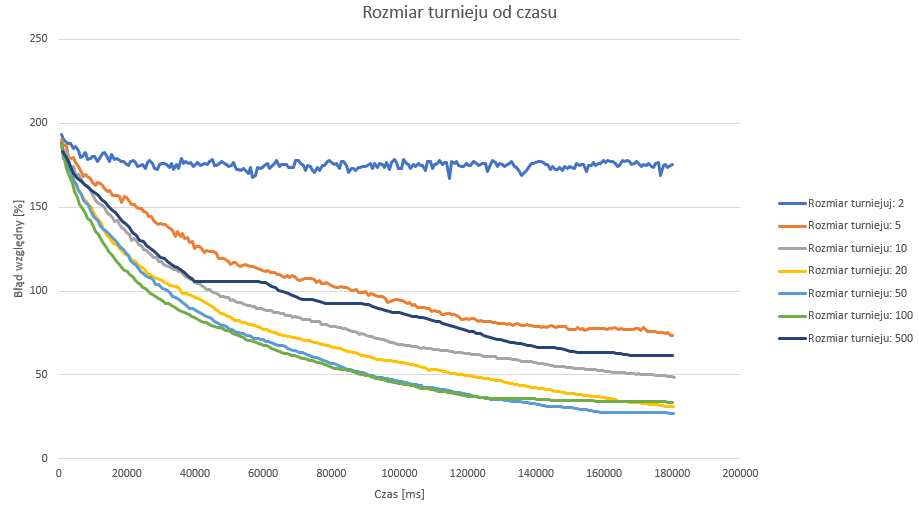
\includegraphics[scale=.58]{tournament.png}%
	\end{adjustbox}
	\begin{adjustbox}{angle=90, center}
	\begin{tabular}{|c|c|}
		\hline
		
		\multicolumn{1}{|c|}{\textbf{Rozm. turnieju}} & \textbf{Błąd wzgl. [\%]}  \\ \hline
		{2}                                	& 175,29               \\ \hline
		{5}                                & 73,38               \\ \hline
		{10}                                & 48,76                 \\ \hline
		{20}                                & 30,91                 \\ \hline
		{50}                                & 27,12                 \\ \hline
		{100}                                & 33,83                 \\ \hline
		{500}                                & 61,58                 \\ \hline		
	\end{tabular}
	
	\end{adjustbox}


\end{figure}

\subsection{Wpływ prawdopodobieństwa wystąpienia mutacji na działanie algorytmu}
\subsubsection{Mutacja Invert}
\begin{figure}[H]
	\begin{adjustbox}{addcode={\begin{minipage}{\width}}{\caption{%
						Wpływ prawdopodobieństwa wystąpienia mutacji typu \textit{invert} na jakość rozwiązania z biegiem czasu. Badania przeprowadzono dla instancji rbg323.
			}\end{minipage}},rotate=90,center}
		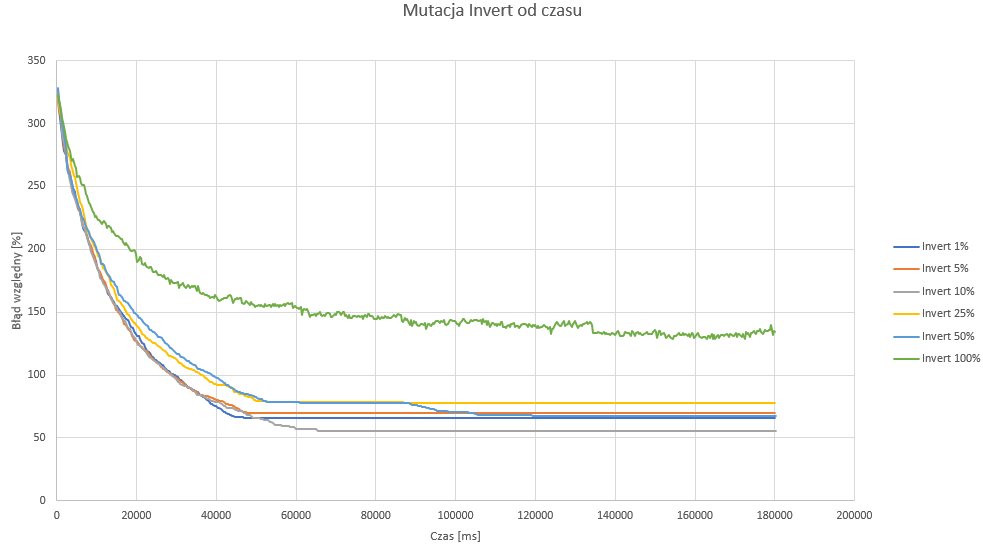
\includegraphics[scale=.53]{invert.png}%
	\end{adjustbox}
\begin{adjustbox}{angle=90, center}
	\begin{tabular}{|c|c|}
		\hline
		
		\multicolumn{1}{|c|}{\textbf{Rozm. turnieju}} & \textbf{Błąd wzgl. [\%]}  \\ \hline
		{1}                                	& 65,61             \\ \hline
		{5}                                & 69,45               \\ \hline
		{10}                                & 55,80                 \\ \hline
		{25}                                & 77,67                \\ \hline
		{50}                                & 67,64                 \\ \hline
		{100}                                & 133,86                 \\ \hline		
	\end{tabular}
	
\end{adjustbox}
\end{figure}

\subsubsection{Mutacja Swap}
\begin{figure}[H]
	\begin{adjustbox}{addcode={\begin{minipage}{\width}}{\caption{%
						Wpływ prawdopodobieństwa wystąpienia mutacji typu \textit{swap} na jakość rozwiązania z biegiem czasu. Badania przeprowadzono dla instancji rbg323.
			}\end{minipage}},rotate=90,center}
		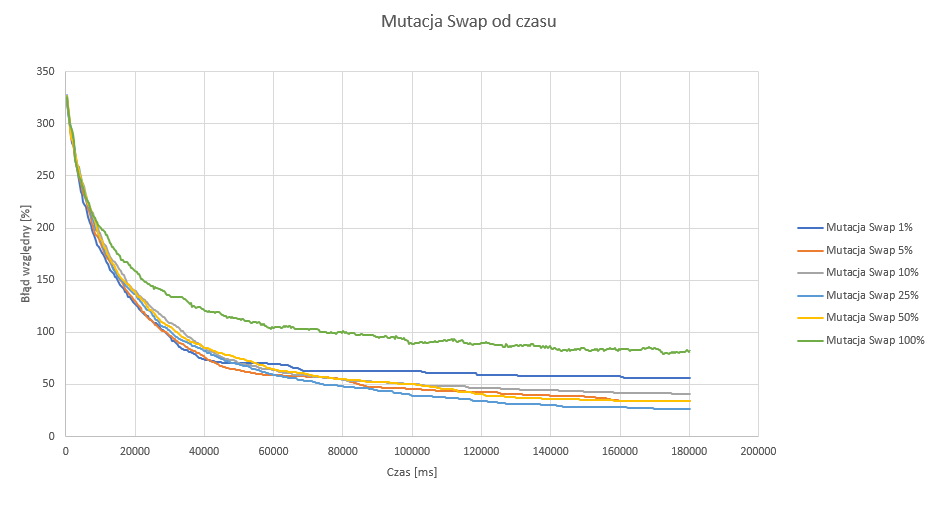
\includegraphics[scale=.59]{swap.png}%
	\end{adjustbox}
\begin{adjustbox}{angle=90, center}
	\begin{tabular}{|c|c|}
		\hline
		
		\multicolumn{1}{|c|}{\textbf{Rozm. turnieju}} & \textbf{Błąd wzgl. [\%]}  \\ \hline
		{1}                                	& 56,03              \\ \hline
		{5}                                & 33,71              \\ \hline
		{10}                                & 41,08                 \\ \hline
		{25}                                & 26,24                 \\ \hline
		{50}                                & 34,17                 \\ \hline
		{100}                                & 82,27                 \\ \hline			
	\end{tabular}
	
\end{adjustbox}
\end{figure}

\newpage	
\section{Podsumowanie}
\par Na podstawie uzyskanych wyników można stwierdzić, iż \textit{Algorytm Genetyczny} z powodzeniem można wykorzystać jako metodę rozwiązywania \textit{TSP}. Nie odbywa się to jednak bez wad: wyniki uzyskane za pomocą tego algorytmu zależą w znacznym stopniu od parametrów(\textit{pkt. 2.2}), jakie zostały dobrane dla danej instancji problemu. Odpowiednie ich wyselekcjonowanie może doprowadzić do uzyskania zadowlających rezultatów - poniżej poziomu 30\% błędu względnego. Istnieje także, katastrofalne w skutkach, ryzyko doboru złych parametrów - w takim przypadku błąd względny może sięgać nawet kilku tysięcy \%.
\\ \par W przeprowadzonych badaniach można zauważyć jak poszczególne parametry wpływają na jakość uzyskanego rozwiązania. Na podstawie otrzymanych wyników wyciągnieto następujące wnioski: rozmiar populacji powinien wynosić ok. 3*rozmiarInstancji, rozmiar populacji macierzystej powinien wynosić połowę rozmiaru populacji, a rozmiar turnieju (jeśli instancja na to pozwala) 
daje najlepsze wyniki dla współczynnika ok. 1/20 *  rozmiar populacji. Mutacja invert, z racji swojej inwazyjności, nie powinna być używana na więcej niż 10\% osobników z danej populacji.

\par
%----------------------------------------------------------------------------------------
%	SECTION 3
%----------------------------------------------------------------------------------------

%----------------------------------------------------------------------------------------
%	SECTION 4
%----------------------------------------------------------------------------------------

%----------------------------------------------------------------------------------------
%	BIBLIOGRAPHY
%----------------------------------------------------------------------------------------
%\newpage
%\bibliohystyle{apalike}
%\begin{thebibliography}{9}
%
%\bibitem{wikipediacluster} 
%Wikipedia: Computer cluster,
%\\\texttt{https://en.wikipedia.org/wiki/Computer\_cluster}
%	
%\bibitem{wikipediasieve} 
%Wikipedia: Sieve of Erastosthenes,
%\\\texttt{https://en.wikipedia.org/wiki/Sieve\_of\_Eratosthenes}
%
%\end{thebibliography}

%----------------------------------------------------------------------------------------
\end{document}
